\documentclass[hyperref={pdfpagelabels=false},12pt]{beamer}
\usepackage[utf8]{inputenc}
%\usepackage{multirow}
%\usepackage{wasysym}
%\usepackage{upquote}
\usepackage{listings}
\usepackage{gensymb}
\usepackage{array}
\usepackage{times}
\usepackage{xcolor}
\usepackage{default}
\usepackage{ulem}

%\usetheme{Pittsburgh}

\xdefinecolor{darkgreen}{rgb}{0.11,0.64,0.22}
\title[Pitt Access]{{\large Pitt ACCESS\\ A Comprehensive and Critical Evaluation System for Software}}
\author[Pitt-Access]{{\scriptsize \textbf{Ketan and Barry}}}
\date{}

\beamertemplatenavigationsymbolsempty


\begin{document}
\begin{frame}[plain]
\titlepage
\end{frame}

%Introduction
\begin{frame}
\frametitle{Motivation}
\begin{itemize}
\itemsep1em
\item 
Frustration with science software: platforms, installation, runtime, maintenance, dependencies
\item 
Diversity: architectures, libraries, tools, compilers
\item 
An independent, neutral and critical evaluation platform: quantitative and qualitative
\end{itemize}
\end{frame}

\begin{frame}
\frametitle{What is it all about?}
\begin{itemize}
\itemsep1em
\item 
A platform to review software: applications, tools, libraries, compiler suites, standards.
\item 
Answers to questions such as:
\begin{itemize}
\item 
I need an MD software for the Nvidia/CUDA platform, which one is the best?
\item 
How well does the new combustion engine simulation software scales at 2048 CPUs?
\item 
Is it worth buying the latest compiler suite from PGI?
\item 
... and many more
\end{itemize}
\end{itemize}

\end{frame}

\begin{frame}
\frametitle{Architecture}
\begin{itemize}
\itemsep1em
\item 
Layered architecture: UI, Test Framework, Evaluation Framework, Storage, DB
\item
Federated: users contribute, review and rate
\item
Record correctness, scalability, compatibility, stability
\item
Structured database for contents
\end{itemize}
\end{frame}

\begin{frame}
\frametitle{Execution: Pipeline}
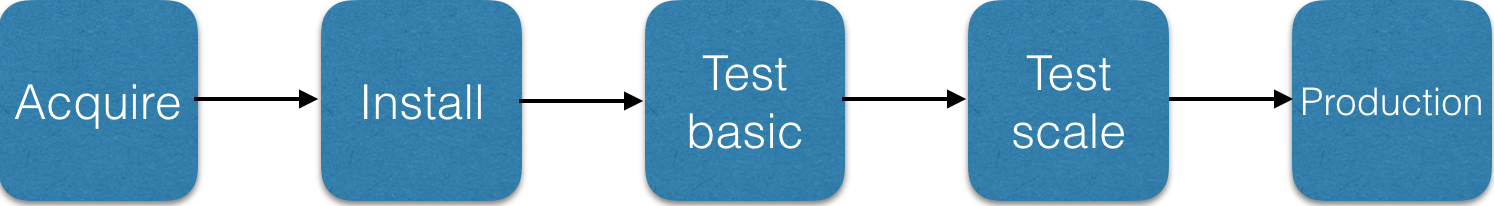
\includegraphics[width=9cm]{workflow}
\end{frame}

\begin{frame}
\frametitle{Challenges}
\begin{itemize}
\itemsep1em
\item
 How do we:
\begin{itemize}
 \item
 measure progress and productivity
 \item
 sustain the effort? funding? infrastructure?
 \item
 What are potential roadblocks?
\end{itemize}
\item 
Strategic: potentially making important people upset
\item
Technological: design, web development
\item
Legal: licensing issues, what to publish and what to withold (start with ``local" software)
\item
Unforeseen: this is a unique and first of its kind effort! (I know everyone says so!)
\end{itemize}
\end{frame}

\begin{frame}
\frametitle{Benefits(1)}
\begin{itemize}
\itemsep1em
\item Strengthen SaM's (and Pitt's) software platforms
\item
Save user's time and money
\item
Strong community outreach elements
\item
Deeper understanding of apps, better collaboration
\end{itemize}
\end{frame}

\begin{frame}
\frametitle{Benefits(2)}
\begin{itemize}
\itemsep1em
\item 
Better information of what the community is up to
\item
Keep in touch with leaders and vice versa
\item
Catalog: tag and locate
\item
Potentially discover new bugs
\end{itemize}
\end{frame}

\begin{frame}
\frametitle{Is it well-aligned to SaM's mission? \\ (Why yes ... yes it is!)}
\begin{itemize}
\itemsep1em
\item 
Promote multi-disciplinary research
\item
Enrich knowledge base
\item
New funding opportunities
\item
Long term: leave a mark!
\end{itemize}
\end{frame}

\begin{frame}
\frametitle{Project Timeline: Medium Term}
\begin{itemize}
\itemsep1em
\item 
Quarter1: incubation, design, tests, feedback
\item
Quarter 2: Narrow down scope, short term goals, select target software, first webpage goes live
\item
Quarter 3: Add more software, diversify science domain
\item
Quarter 4:
\item
Year 2?
\item
Year 3?
\end{itemize}
\end{frame}

\begin{frame}
\frametitle{Project Timeline: Short Term}
\begin{itemize}
\itemsep1em
\item 
Next month
\item
Select 2-3 software apps
\item
Perform the acquire, install, test, run, scale cycle
\item
Identify and register patterns, eg. effort to install
\item
Tools to build the platform: django/flask?, sqlite3?, json?, ...
\end{itemize}
\end{frame}

\begin{frame}
\frametitle{Long Term}
\begin{itemize}
\item 
establish a ``center"
\end{itemize}
\end{frame}

\begin{frame}
\frametitle{Summary}
\begin{itemize}
\itemsep1em
\item IMDb of science software!
\item
A critical and comprehensive evaluation platform for software will enable better usage of science software
\item
Valuable at all scales, many fringe benefits, strong elements of outreach
\item
Contribution to multi-disciplinary software infrastructure
\end{itemize}
\end{frame}

\begin{frame}
\frametitle{Questions}
\begin{itemize}
\item We are looking for critical comments and feedback!
\end{itemize}
\end{frame}

\end{document}

